\documentclass[1p]{elsarticle_modified}
%\bibliographystyle{elsarticle-num}

%\usepackage[colorlinks]{hyperref}
%\usepackage{abbrmath_seonhwa} %\Abb, \Ascr, \Acal ,\Abf, \Afrak
\usepackage{amsfonts}
\usepackage{amssymb}
\usepackage{amsmath}
\usepackage{amsthm}
\usepackage{scalefnt}
\usepackage{amsbsy}
\usepackage{kotex}
\usepackage{caption}
\usepackage{subfig}
\usepackage{color}
\usepackage{graphicx}
\usepackage{xcolor} %% white, black, red, green, blue, cyan, magenta, yellow
\usepackage{float}
\usepackage{setspace}
\usepackage{hyperref}

\usepackage{tikz}
\usetikzlibrary{arrows}

\usepackage{multirow}
\usepackage{array} % fixed length table
\usepackage{hhline}

%%%%%%%%%%%%%%%%%%%%%
\makeatletter
\renewcommand*\env@matrix[1][\arraystretch]{%
	\edef\arraystretch{#1}%
	\hskip -\arraycolsep
	\let\@ifnextchar\new@ifnextchar
	\array{*\c@MaxMatrixCols c}}
\makeatother %https://tex.stackexchange.com/questions/14071/how-can-i-increase-the-line-spacing-in-a-matrix
%%%%%%%%%%%%%%%

\usepackage[normalem]{ulem}

\newcommand{\msout}[1]{\ifmmode\text{\sout{\ensuremath{#1}}}\else\sout{#1}\fi}
%SOURCE: \msout is \stkout macro in https://tex.stackexchange.com/questions/20609/strikeout-in-math-mode

\newcommand{\cancel}[1]{
	\ifmmode
	{\color{red}\msout{#1}}
	\else
	{\color{red}\sout{#1}}
	\fi
}

\newcommand{\add}[1]{
	{\color{blue}\uwave{#1}}
}

\newcommand{\replace}[2]{
	\ifmmode
	{\color{red}\msout{#1}}{\color{blue}\uwave{#2}}
	\else
	{\color{red}\sout{#1}}{\color{blue}\uwave{#2}}
	\fi
}

\newcommand{\Sol}{\mathcal{S}} %segment
\newcommand{\D}{D} %diagram
\newcommand{\A}{\mathcal{A}} %arc


%%%%%%%%%%%%%%%%%%%%%%%%%%%%%5 test

\def\sl{\operatorname{\textup{SL}}(2,\Cbb)}
\def\psl{\operatorname{\textup{PSL}}(2,\Cbb)}
\def\quan{\mkern 1mu \triangleright \mkern 1mu}

\theoremstyle{definition}
\newtheorem{thm}{Theorem}[section]
\newtheorem{prop}[thm]{Proposition}
\newtheorem{lem}[thm]{Lemma}
\newtheorem{ques}[thm]{Question}
\newtheorem{cor}[thm]{Corollary}
\newtheorem{defn}[thm]{Definition}
\newtheorem{exam}[thm]{Example}
\newtheorem{rmk}[thm]{Remark}
\newtheorem{alg}[thm]{Algorithm}

\newcommand{\I}{\sqrt{-1}}
\begin{document}

%\begin{frontmatter}
%
%\title{Boundary parabolic representations of knots up to 8 crossings}
%
%%% Group authors per affiliation:
%\author{Yunhi Cho} 
%\address{Department of Mathematics, University of Seoul, Seoul, Korea}
%\ead{yhcho@uos.ac.kr}
%
%
%\author{Seonhwa Kim} %\fnref{s_kim}}
%\address{Center for Geometry and Physics, Institute for Basic Science, Pohang, 37673, Korea}
%\ead{ryeona17@ibs.re.kr}
%
%\author{Hyuk Kim}
%\address{Department of Mathematical Sciences, Seoul National University, Seoul 08826, Korea}
%\ead{hyukkim@snu.ac.kr}
%
%\author{Seokbeom Yoon}
%\address{Department of Mathematical Sciences, Seoul National University, Seoul, 08826,  Korea}
%\ead{sbyoon15@snu.ac.kr}
%
%\begin{abstract}
%We find all boundary parabolic representation of knots up to 8 crossings.
%
%\end{abstract}
%\begin{keyword}
%    \MSC[2010] 57M25 
%\end{keyword}
%
%\end{frontmatter}

%\linenumbers
%\tableofcontents
%
\newcommand\colored[1]{\textcolor{white}{\rule[-0.35ex]{0.8em}{1.4ex}}\kern-0.8em\color{red} #1}%
%\newcommand\colored[1]{\textcolor{white}{ #1}\kern-2.17ex	\textcolor{white}{ #1}\kern-1.81ex	\textcolor{white}{ #1}\kern-2.15ex\color{red}#1	}

{\Large $\underline{11a_{21}~(K11a_{21})}$}

\setlength{\tabcolsep}{10pt}
\renewcommand{\arraystretch}{1.6}
\vspace{1cm}\begin{tabular}{m{100pt}>{\centering\arraybackslash}m{274pt}}
\multirow{5}{120pt}{
	\centering
	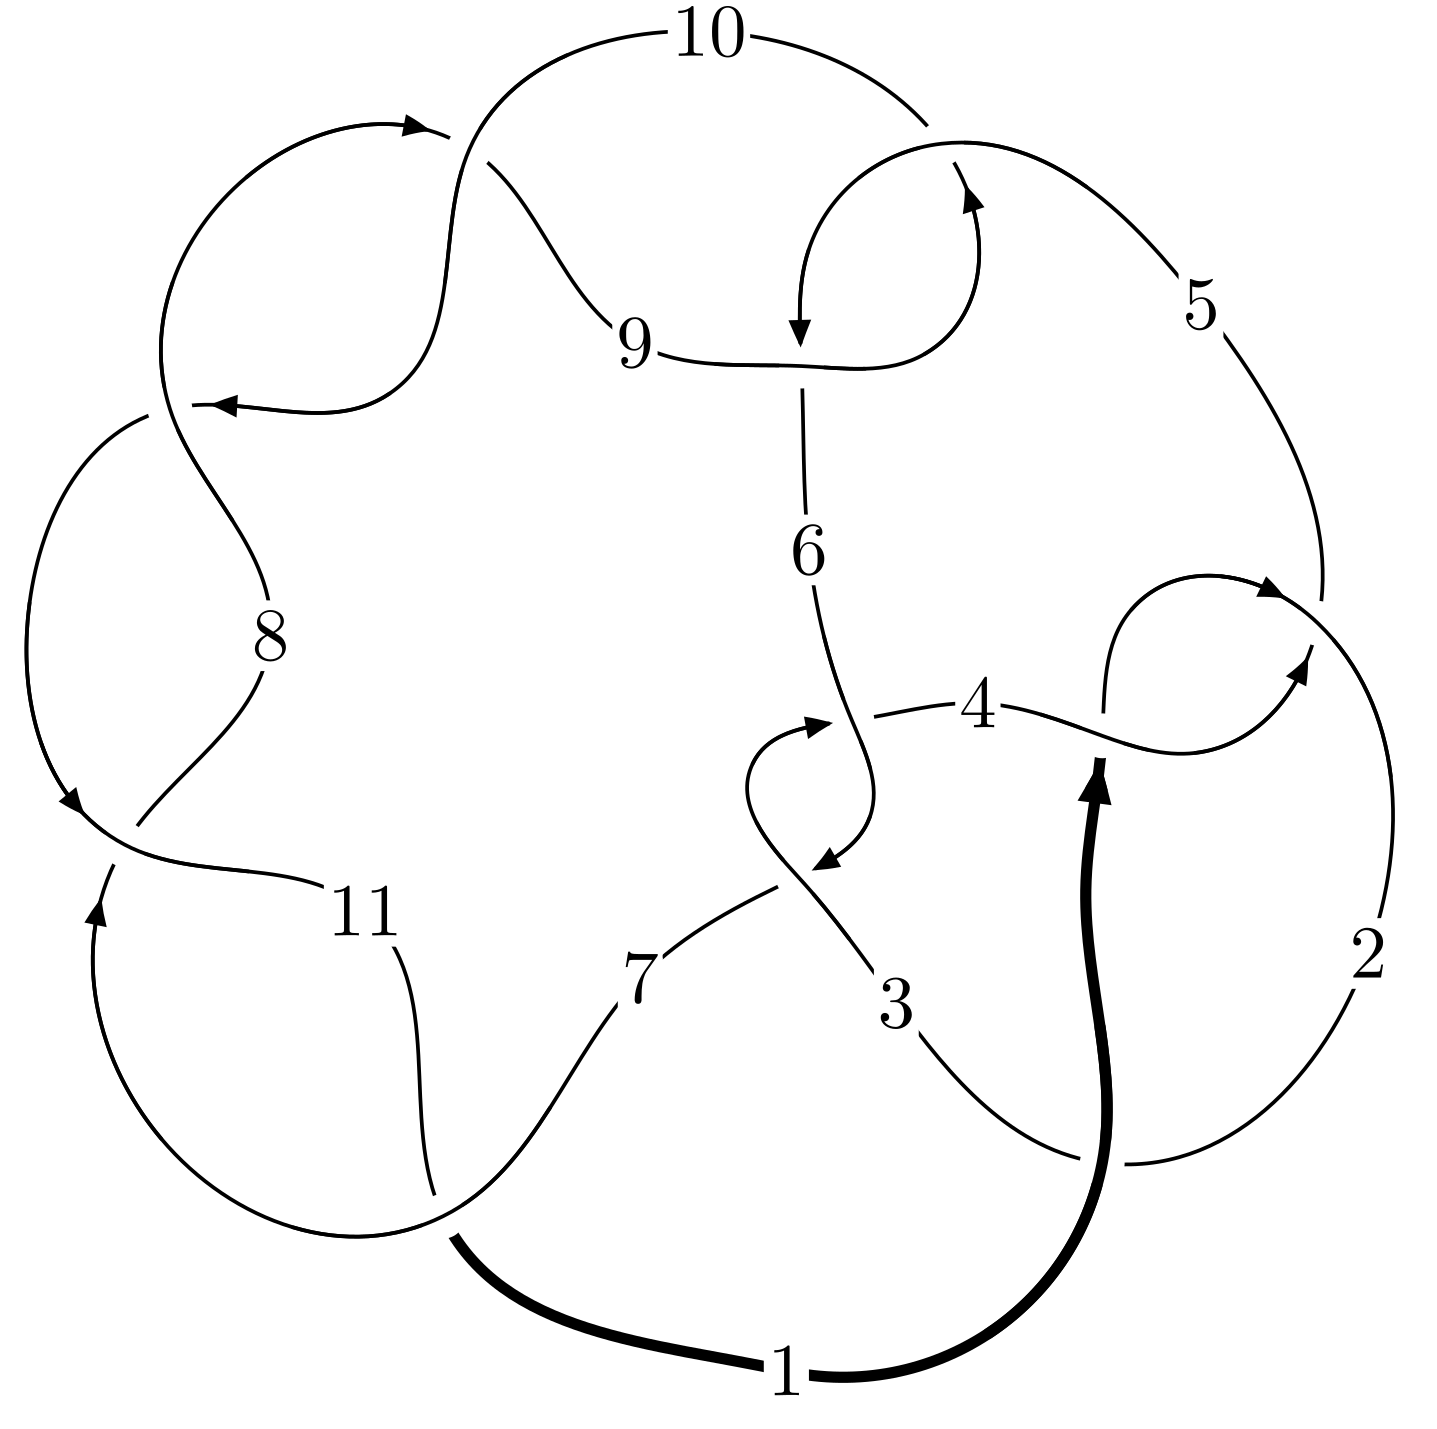
\includegraphics[width=112pt]{../../../GIT/diagram.site/Diagrams/png/270_11a_21.png}\\
\ \ \ A knot diagram\footnotemark}&
\allowdisplaybreaks
\textbf{Linearized knot diagam} \\
\cline{2-2}
 &
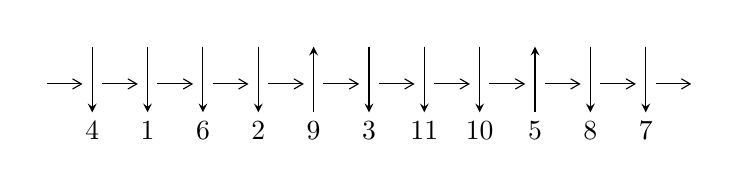
\begin{tikzpicture}[x=20pt, y=17pt]
	% nodes
	\node (C0) at (0, 0) {};
	\node (C1) at (1, 0) {};
	\node (C1U) at (1, +1) {};
	\node (C1D) at (1, -1) {4};

	\node (C2) at (2, 0) {};
	\node (C2U) at (2, +1) {};
	\node (C2D) at (2, -1) {1};

	\node (C3) at (3, 0) {};
	\node (C3U) at (3, +1) {};
	\node (C3D) at (3, -1) {6};

	\node (C4) at (4, 0) {};
	\node (C4U) at (4, +1) {};
	\node (C4D) at (4, -1) {2};

	\node (C5) at (5, 0) {};
	\node (C5U) at (5, +1) {};
	\node (C5D) at (5, -1) {9};

	\node (C6) at (6, 0) {};
	\node (C6U) at (6, +1) {};
	\node (C6D) at (6, -1) {3};

	\node (C7) at (7, 0) {};
	\node (C7U) at (7, +1) {};
	\node (C7D) at (7, -1) {11};

	\node (C8) at (8, 0) {};
	\node (C8U) at (8, +1) {};
	\node (C8D) at (8, -1) {10};

	\node (C9) at (9, 0) {};
	\node (C9U) at (9, +1) {};
	\node (C9D) at (9, -1) {5};

	\node (C10) at (10, 0) {};
	\node (C10U) at (10, +1) {};
	\node (C10D) at (10, -1) {8};

	\node (C11) at (11, 0) {};
	\node (C11U) at (11, +1) {};
	\node (C11D) at (11, -1) {7};
	\node (C12) at (12, 0) {};

	% arrows
	\draw[->,>={angle 60}]
	(C0) edge (C1) (C1) edge (C2) (C2) edge (C3) (C3) edge (C4) (C4) edge (C5) (C5) edge (C6) (C6) edge (C7) (C7) edge (C8) (C8) edge (C9) (C9) edge (C10) (C10) edge (C11) (C11) edge (C12) ;	\draw[->,>=stealth]
	(C1U) edge (C1D) (C2U) edge (C2D) (C3U) edge (C3D) (C4U) edge (C4D) (C5D) edge (C5U) (C6U) edge (C6D) (C7U) edge (C7D) (C8U) edge (C8D) (C9D) edge (C9U) (C10U) edge (C10D) (C11U) edge (C11D) ;
	\end{tikzpicture} \\
\hhline{~~} \\& 
\textbf{Solving Sequence} \\ \cline{2-2} 
 &
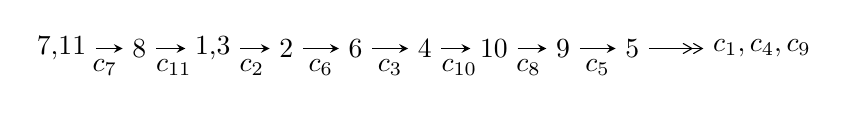
\begin{tikzpicture}[x=25pt, y=7pt]
	% node
	\node (A0) at (-1/8, 0) {7,11};
	\node (A1) at (1, 0) {8};
	\node (A2) at (33/16, 0) {1,3};
	\node (A3) at (25/8, 0) {2};
	\node (A4) at (33/8, 0) {6};
	\node (A5) at (41/8, 0) {4};
	\node (A6) at (49/8, 0) {10};
	\node (A7) at (57/8, 0) {9};
	\node (A8) at (65/8, 0) {5};
	\node (C1) at (1/2, -1) {$c_{7}$};
	\node (C2) at (3/2, -1) {$c_{11}$};
	\node (C3) at (21/8, -1) {$c_{2}$};
	\node (C4) at (29/8, -1) {$c_{6}$};
	\node (C5) at (37/8, -1) {$c_{3}$};
	\node (C6) at (45/8, -1) {$c_{10}$};
	\node (C7) at (53/8, -1) {$c_{8}$};
	\node (C8) at (61/8, -1) {$c_{5}$};
	\node (A9) at (10, 0) {$c_{1},c_{4},c_{9}$};

	% edge
	\draw[->,>=stealth]	
	(A0) edge (A1) (A1) edge (A2) (A2) edge (A3) (A3) edge (A4) (A4) edge (A5) (A5) edge (A6) (A6) edge (A7) (A7) edge (A8) ;
	\draw[->>,>={angle 60}]	
	(A8) edge (A9);
\end{tikzpicture} \\ 

\end{tabular} \\

\footnotetext{
The image of knot diagram is generated by the software ``\textbf{Draw programme}" developed by Andrew Bartholomew(\url{http://www.layer8.co.uk/maths/draw/index.htm\#Running-draw}), where we modified some parts for our purpose(\url{https://github.com/CATsTAILs/LinksPainter}).
}\phantom \\ \newline 
\centering \textbf{Ideals for irreducible components\footnotemark of $X_{\text{par}}$} 
 
\begin{align*}
I^u_{1}&=\langle 
1428543776353 u^{40}+10013523822393 u^{39}+\cdots+2380906293938 b-13661168161,\\
\phantom{I^u_{1}}&\phantom{= \langle  }-857126265809 u^{40}-5059671029533 u^{39}+\cdots+2380906293938 a+15522003749453,\\
\phantom{I^u_{1}}&\phantom{= \langle  }u^{41}+8 u^{40}+\cdots+9 u-1\rangle \\
I^u_{2}&=\langle 
b,\;- u^3+u^2+a-3 u+2,\;u^4- u^3+3 u^2-2 u+1\rangle \\
\\
\end{align*}
\raggedright * 2 irreducible components of $\dim_{\mathbb{C}}=0$, with total 45 representations.\\
\footnotetext{All coefficients of polynomials are rational numbers. But the coefficients are sometimes approximated in decimal forms when there is not enough margin.}
\newpage
\renewcommand{\arraystretch}{1}
\centering \section*{I. $I^u_{1}= \langle 1.43\times10^{12} u^{40}+1.00\times10^{13} u^{39}+\cdots+2.38\times10^{12} b-1.37\times10^{10},\;-8.57\times10^{11} u^{40}-5.06\times10^{12} u^{39}+\cdots+2.38\times10^{12} a+1.55\times10^{13},\;u^{41}+8 u^{40}+\cdots+9 u-1 \rangle$}
\flushleft \textbf{(i) Arc colorings}\\
\begin{tabular}{m{7pt} m{180pt} m{7pt} m{180pt} }
\flushright $a_{7}=$&$\begin{pmatrix}1\\0\end{pmatrix}$ \\
\flushright $a_{11}=$&$\begin{pmatrix}0\\u\end{pmatrix}$ \\
\flushright $a_{8}=$&$\begin{pmatrix}1\\u^2\end{pmatrix}$ \\
\flushright $a_{1}=$&$\begin{pmatrix}- u\\u\end{pmatrix}$ \\
\flushright $a_{3}=$&$\begin{pmatrix}0.360000 u^{40}+2.12510 u^{39}+\cdots-57.3965 u-6.51937\\-0.600000 u^{40}-4.20576 u^{39}+\cdots-5.97164 u+0.00573780\end{pmatrix}$ \\
\flushright $a_{2}=$&$\begin{pmatrix}0.160000 u^{40}+0.886423 u^{39}+\cdots-56.1906 u-6.68003\\-0.400000 u^{40}-2.96708 u^{39}+\cdots-7.17757 u+0.166396\end{pmatrix}$ \\
\flushright $a_{6}=$&$\begin{pmatrix}-0.604092 u^{40}-5.23273 u^{39}+\cdots-27.0571 u-2.48000\\0.598354 u^{40}+4.78683 u^{39}+\cdots+2.11593 u-0.600000\end{pmatrix}$ \\
\flushright $a_{4}=$&$\begin{pmatrix}0.160000 u^{40}+0.668312 u^{39}+\cdots-66.4027 u-8.31995\\-0.600000 u^{40}-4.14815 u^{39}+\cdots-7.25524 u-0.0516402\end{pmatrix}$ \\
\flushright $a_{10}=$&$\begin{pmatrix}u\\u^3+u\end{pmatrix}$ \\
\flushright $a_{9}=$&$\begin{pmatrix}u^2+1\\u^4+2 u^2\end{pmatrix}$ \\
\flushright $a_{5}=$&$\begin{pmatrix}-0.200000 u^{40}-2.00411 u^{39}+\cdots-22.3773 u-2.67998\\-0.400000 u^{40}-2.19754 u^{39}+\cdots+2.95683 u-0.604092\end{pmatrix}$\\ \flushright $a_{5}=$&$\begin{pmatrix}-0.200000 u^{40}-2.00411 u^{39}+\cdots-22.3773 u-2.67998\\-0.400000 u^{40}-2.19754 u^{39}+\cdots+2.95683 u-0.604092\end{pmatrix}$\\&\end{tabular}
\flushleft \textbf{(ii) Obstruction class $= -1$}\\~\\
\flushleft \textbf{(iii) Cusp Shapes $= \frac{3866826976577}{1190453146969} u^{40}+\frac{30172725798597}{1190453146969} u^{39}+\cdots+\frac{97267270764267}{1190453146969} u-\frac{19437718983710}{1190453146969}$}\\~\\
\newpage\renewcommand{\arraystretch}{1}
\flushleft \textbf{(iv) u-Polynomials at the component}\newline \\
\begin{tabular}{m{50pt}|m{274pt}}
Crossings & \hspace{64pt}u-Polynomials at each crossing \\
\hline $$\begin{aligned}c_{1},c_{4}\end{aligned}$$&$\begin{aligned}
&u^{41}-5 u^{40}+\cdots-7 u+1
\end{aligned}$\\
\hline $$\begin{aligned}c_{2}\end{aligned}$$&$\begin{aligned}
&u^{41}+17 u^{40}+\cdots-21 u+1
\end{aligned}$\\
\hline $$\begin{aligned}c_{3},c_{6}\end{aligned}$$&$\begin{aligned}
&u^{41}- u^{40}+\cdots+24 u+16
\end{aligned}$\\
\hline $$\begin{aligned}c_{5},c_{9}\end{aligned}$$&$\begin{aligned}
&u^{41}-2 u^{40}+\cdots+u+1
\end{aligned}$\\
\hline $$\begin{aligned}c_{7},c_{8},c_{10}\\c_{11}\end{aligned}$$&$\begin{aligned}
&u^{41}+8 u^{40}+\cdots+9 u-1
\end{aligned}$\\
\hline
\end{tabular}\\~\\
\newpage\renewcommand{\arraystretch}{1}
\flushleft \textbf{(v) Riley Polynomials at the component}\newline \\
\begin{tabular}{m{50pt}|m{274pt}}
Crossings & \hspace{64pt}Riley Polynomials at each crossing \\
\hline $$\begin{aligned}c_{1},c_{4}\end{aligned}$$&$\begin{aligned}
&y^{41}-17 y^{40}+\cdots-21 y-1
\end{aligned}$\\
\hline $$\begin{aligned}c_{2}\end{aligned}$$&$\begin{aligned}
&y^{41}+19 y^{40}+\cdots+319 y-1
\end{aligned}$\\
\hline $$\begin{aligned}c_{3},c_{6}\end{aligned}$$&$\begin{aligned}
&y^{41}+27 y^{40}+\cdots-3264 y-256
\end{aligned}$\\
\hline $$\begin{aligned}c_{5},c_{9}\end{aligned}$$&$\begin{aligned}
&y^{41}+8 y^{40}+\cdots+9 y-1
\end{aligned}$\\
\hline $$\begin{aligned}c_{7},c_{8},c_{10}\\c_{11}\end{aligned}$$&$\begin{aligned}
&y^{41}+52 y^{40}+\cdots+289 y-1
\end{aligned}$\\
\hline
\end{tabular}\\~\\
\newpage\flushleft \textbf{(vi) Complex Volumes and Cusp Shapes}
$$\begin{array}{c|c|c}  
\text{Solutions to }I^u_{1}& \I (\text{vol} + \sqrt{-1}CS) & \text{Cusp shape}\\
 \hline 
\begin{aligned}
u &= -0.371997 + 0.911661 I \\
a &= \phantom{-}0.0887599 - 0.0951085 I \\
b &= \phantom{-}0.944034 + 0.301769 I\end{aligned}
 & \phantom{-}0.02027 + 4.12007 I & -7.00000 - 7.00432 I \\ \hline\begin{aligned}
u &= -0.371997 - 0.911661 I \\
a &= \phantom{-}0.0887599 + 0.0951085 I \\
b &= \phantom{-}0.944034 - 0.301769 I\end{aligned}
 & \phantom{-}0.02027 - 4.12007 I & -7.00000 + 7.00432 I \\ \hline\begin{aligned}
u &= \phantom{-}0.123662 + 0.937506 I \\
a &= \phantom{-}0.94133 - 1.41174 I \\
b &= \phantom{-}0.152966 + 1.275670 I\end{aligned}
 & \phantom{-}5.54405 + 0.90504 I & \phantom{-0.000000 } 0. - 2.30521 I \\ \hline\begin{aligned}
u &= \phantom{-}0.123662 - 0.937506 I \\
a &= \phantom{-}0.94133 + 1.41174 I \\
b &= \phantom{-}0.152966 - 1.275670 I\end{aligned}
 & \phantom{-}5.54405 - 0.90504 I & \phantom{-0.000000 -}0. + 2.30521 I \\ \hline\begin{aligned}
u &= -0.744727 + 0.518203 I \\
a &= -0.330115 - 0.059884 I \\
b &= \phantom{-}0.127427 + 0.966899 I\end{aligned}
 & -0.343144 + 0.381292 I & -7.00000 + 0. I\phantom{ +0.000000I} \\ \hline\begin{aligned}
u &= -0.744727 - 0.518203 I \\
a &= -0.330115 + 0.059884 I \\
b &= \phantom{-}0.127427 - 0.966899 I\end{aligned}
 & -0.343144 - 0.381292 I & -7.00000 + 0. I\phantom{ +0.000000I} \\ \hline\begin{aligned}
u &= -0.860587 + 0.281389 I \\
a &= \phantom{-}0.620418 + 0.125659 I \\
b &= \phantom{-}0.383866 - 1.083520 I\end{aligned}
 & -1.07493 + 4.80769 I & -9.34122 - 6.74048 I \\ \hline\begin{aligned}
u &= -0.860587 - 0.281389 I \\
a &= \phantom{-}0.620418 - 0.125659 I \\
b &= \phantom{-}0.383866 + 1.083520 I\end{aligned}
 & -1.07493 - 4.80769 I & -9.34122 + 6.74048 I \\ \hline\begin{aligned}
u &= \phantom{-}0.250188 + 0.801720 I \\
a &= -1.38496 + 1.41699 I \\
b &= -0.452932 - 1.292530 I\end{aligned}
 & \phantom{-}4.35267 - 4.76438 I & -1.23872 + 3.17616 I \\ \hline\begin{aligned}
u &= \phantom{-}0.250188 - 0.801720 I \\
a &= -1.38496 - 1.41699 I \\
b &= -0.452932 + 1.292530 I\end{aligned}
 & \phantom{-}4.35267 + 4.76438 I & -1.23872 - 3.17616 I\\
 \hline 
 \end{array}$$\newpage$$\begin{array}{c|c|c}  
\text{Solutions to }I^u_{1}& \I (\text{vol} + \sqrt{-1}CS) & \text{Cusp shape}\\
 \hline 
\begin{aligned}
u &= -0.298760 + 0.775703 I \\
a &= \phantom{-}0.30126 + 2.51541 I \\
b &= \phantom{-}0.152801 - 0.776585 I\end{aligned}
 & -1.09017 + 1.98652 I & -2.92718 - 5.89159 I \\ \hline\begin{aligned}
u &= -0.298760 - 0.775703 I \\
a &= \phantom{-}0.30126 - 2.51541 I \\
b &= \phantom{-}0.152801 + 0.776585 I\end{aligned}
 & -1.09017 - 1.98652 I & -2.92718 + 5.89159 I \\ \hline\begin{aligned}
u &= -0.402696 + 1.111770 I \\
a &= -0.448898 - 1.278070 I \\
b &= -0.300924 + 1.194930 I\end{aligned}
 & \phantom{-}4.72505 + 4.10019 I & \phantom{-0.000000 } 0 \\ \hline\begin{aligned}
u &= -0.402696 - 1.111770 I \\
a &= -0.448898 + 1.278070 I \\
b &= -0.300924 - 1.194930 I\end{aligned}
 & \phantom{-}4.72505 - 4.10019 I & \phantom{-0.000000 } 0 \\ \hline\begin{aligned}
u &= -0.563543 + 1.076360 I \\
a &= \phantom{-}0.77154 + 1.22276 I \\
b &= \phantom{-}0.544305 - 1.241970 I\end{aligned}
 & \phantom{-}3.04149 + 9.59886 I & \phantom{-0.000000 } 0 \\ \hline\begin{aligned}
u &= -0.563543 - 1.076360 I \\
a &= \phantom{-}0.77154 - 1.22276 I \\
b &= \phantom{-}0.544305 + 1.241970 I\end{aligned}
 & \phantom{-}3.04149 - 9.59886 I & \phantom{-0.000000 } 0 \\ \hline\begin{aligned}
u &= -0.094895 + 0.764233 I \\
a &= \phantom{-}0.081309 + 0.430953 I \\
b &= -0.903364 + 0.108240 I\end{aligned}
 & \phantom{-}0.550320 + 0.199179 I & -3.56736 - 0.22812 I \\ \hline\begin{aligned}
u &= -0.094895 - 0.764233 I \\
a &= \phantom{-}0.081309 - 0.430953 I \\
b &= -0.903364 - 0.108240 I\end{aligned}
 & \phantom{-}0.550320 - 0.199179 I & -3.56736 + 0.22812 I \\ \hline\begin{aligned}
u &= -0.560839 + 0.097240 I \\
a &= \phantom{-}1.30596 - 1.04621 I \\
b &= \phantom{-}0.579988 + 0.456802 I\end{aligned}
 & -3.06538 + 0.92602 I & -14.9814 - 0.1523 I \\ \hline\begin{aligned}
u &= -0.560839 - 0.097240 I \\
a &= \phantom{-}1.30596 + 1.04621 I \\
b &= \phantom{-}0.579988 - 0.456802 I\end{aligned}
 & -3.06538 - 0.92602 I & -14.9814 + 0.1523 I\\
 \hline 
 \end{array}$$\newpage$$\begin{array}{c|c|c}  
\text{Solutions to }I^u_{1}& \I (\text{vol} + \sqrt{-1}CS) & \text{Cusp shape}\\
 \hline 
\begin{aligned}
u &= -0.369951 + 0.353558 I \\
a &= \phantom{-}0.185674 - 0.401147 I \\
b &= -0.276914 + 0.386438 I\end{aligned}
 & -0.304070 + 1.129050 I & -4.15006 - 5.99735 I \\ \hline\begin{aligned}
u &= -0.369951 - 0.353558 I \\
a &= \phantom{-}0.185674 + 0.401147 I \\
b &= -0.276914 - 0.386438 I\end{aligned}
 & -0.304070 - 1.129050 I & -4.15006 + 5.99735 I \\ \hline\begin{aligned}
u &= -0.12602 + 1.51041 I \\
a &= -0.013258 - 0.326775 I \\
b &= \phantom{-}0.008065 + 0.612774 I\end{aligned}
 & \phantom{-}5.86173 + 3.10796 I & \phantom{-0.000000 } 0 \\ \hline\begin{aligned}
u &= -0.12602 - 1.51041 I \\
a &= -0.013258 + 0.326775 I \\
b &= \phantom{-}0.008065 - 0.612774 I\end{aligned}
 & \phantom{-}5.86173 - 3.10796 I & \phantom{-0.000000 } 0 \\ \hline\begin{aligned}
u &= \phantom{-}0.379955 + 0.102142 I \\
a &= \phantom{-}0.22338 + 1.77156 I \\
b &= -0.210011 + 1.175300 I\end{aligned}
 & \phantom{-}2.27591 + 2.55277 I & -0.28600 - 3.41736 I \\ \hline\begin{aligned}
u &= \phantom{-}0.379955 - 0.102142 I \\
a &= \phantom{-}0.22338 - 1.77156 I \\
b &= -0.210011 - 1.175300 I\end{aligned}
 & \phantom{-}2.27591 - 2.55277 I & -0.28600 + 3.41736 I \\ \hline\begin{aligned}
u &= -0.06786 + 1.66115 I \\
a &= \phantom{-}0.00695 + 2.26459 I \\
b &= \phantom{-}0.022295 - 1.118440 I\end{aligned}
 & \phantom{-}7.48443 + 3.29627 I & \phantom{-0.000000 } 0 \\ \hline\begin{aligned}
u &= -0.06786 - 1.66115 I \\
a &= \phantom{-}0.00695 - 2.26459 I \\
b &= \phantom{-}0.022295 + 1.118440 I\end{aligned}
 & \phantom{-}7.48443 - 3.29627 I & \phantom{-0.000000 } 0 \\ \hline\begin{aligned}
u &= -0.02762 + 1.66408 I \\
a &= \phantom{-}0.518524 - 0.032043 I \\
b &= -1.212440 + 0.190127 I\end{aligned}
 & \phantom{-}9.18847 + 0.68171 I & \phantom{-0.000000 } 0 \\ \hline\begin{aligned}
u &= -0.02762 - 1.66408 I \\
a &= \phantom{-}0.518524 + 0.032043 I \\
b &= -1.212440 - 0.190127 I\end{aligned}
 & \phantom{-}9.18847 - 0.68171 I & \phantom{-0.000000 } 0\\
 \hline 
 \end{array}$$\newpage$$\begin{array}{c|c|c}  
\text{Solutions to }I^u_{1}& \I (\text{vol} + \sqrt{-1}CS) & \text{Cusp shape}\\
 \hline 
\begin{aligned}
u &= \phantom{-}0.06444 + 1.66622 I \\
a &= -0.40564 + 1.80984 I \\
b &= -0.63341 - 1.39654 I\end{aligned}
 & \phantom{-}13.0504 - 5.9463 I & \phantom{-0.000000 } 0 \\ \hline\begin{aligned}
u &= \phantom{-}0.06444 - 1.66622 I \\
a &= -0.40564 - 1.80984 I \\
b &= -0.63341 + 1.39654 I\end{aligned}
 & \phantom{-}13.0504 + 5.9463 I & \phantom{-0.000000 } 0 \\ \hline\begin{aligned}
u &= -0.09721 + 1.68666 I \\
a &= -0.502494 - 0.093711 I \\
b &= \phantom{-}1.213200 + 0.228523 I\end{aligned}
 & \phantom{-}9.10647 + 5.94562 I & \phantom{-0.000000 } 0 \\ \hline\begin{aligned}
u &= -0.09721 - 1.68666 I \\
a &= -0.502494 + 0.093711 I \\
b &= \phantom{-}1.213200 - 0.228523 I\end{aligned}
 & \phantom{-}9.10647 - 5.94562 I & \phantom{-0.000000 } 0 \\ \hline\begin{aligned}
u &= \phantom{-}0.02231 + 1.69742 I \\
a &= \phantom{-}0.26842 - 1.88152 I \\
b &= \phantom{-}0.37989 + 1.47255 I\end{aligned}
 & \phantom{-}14.9053 + 0.3952 I & \phantom{-0.000000 } 0 \\ \hline\begin{aligned}
u &= \phantom{-}0.02231 - 1.69742 I \\
a &= \phantom{-}0.26842 + 1.88152 I \\
b &= \phantom{-}0.37989 - 1.47255 I\end{aligned}
 & \phantom{-}14.9053 - 0.3952 I & \phantom{-0.000000 } 0 \\ \hline\begin{aligned}
u &= -0.11803 + 1.73749 I \\
a &= -0.21725 - 1.84068 I \\
b &= -0.41152 + 1.45863 I\end{aligned}
 & \phantom{-}14.7445 + 6.3325 I & \phantom{-0.000000 } 0 \\ \hline\begin{aligned}
u &= -0.11803 - 1.73749 I \\
a &= -0.21725 + 1.84068 I \\
b &= -0.41152 - 1.45863 I\end{aligned}
 & \phantom{-}14.7445 - 6.3325 I & \phantom{-0.000000 } 0 \\ \hline\begin{aligned}
u &= -0.16530 + 1.73400 I \\
a &= \phantom{-}0.35701 + 1.74321 I \\
b &= \phantom{-}0.65439 - 1.38049 I\end{aligned}
 & \phantom{-}12.7852 + 12.6394 I & \phantom{-0.000000 } 0 \\ \hline\begin{aligned}
u &= -0.16530 - 1.73400 I \\
a &= \phantom{-}0.35701 - 1.74321 I \\
b &= \phantom{-}0.65439 + 1.38049 I\end{aligned}
 & \phantom{-}12.7852 - 12.6394 I & \phantom{-0.000000 } 0\\
 \hline 
 \end{array}$$\newpage$$\begin{array}{c|c|c}  
\text{Solutions to }I^u_{1}& \I (\text{vol} + \sqrt{-1}CS) & \text{Cusp shape}\\
 \hline 
\begin{aligned}
u &= \phantom{-}0.0589447\phantom{ +0.000000I} \\
a &= -10.7359\phantom{ +0.000000I} \\
b &= -0.523441\phantom{ +0.000000I}\end{aligned}
 & -1.19034\phantom{ +0.000000I} & -8.28720\phantom{ +0.000000I}\\
 \hline 
 \end{array}$$\newpage\newpage\renewcommand{\arraystretch}{1}
\centering \section*{II. $I^u_{2}= \langle b,\;- u^3+u^2+a-3 u+2,\;u^4- u^3+3 u^2-2 u+1 \rangle$}
\flushleft \textbf{(i) Arc colorings}\\
\begin{tabular}{m{7pt} m{180pt} m{7pt} m{180pt} }
\flushright $a_{7}=$&$\begin{pmatrix}1\\0\end{pmatrix}$ \\
\flushright $a_{11}=$&$\begin{pmatrix}0\\u\end{pmatrix}$ \\
\flushright $a_{8}=$&$\begin{pmatrix}1\\u^2\end{pmatrix}$ \\
\flushright $a_{1}=$&$\begin{pmatrix}- u\\u\end{pmatrix}$ \\
\flushright $a_{3}=$&$\begin{pmatrix}u^3- u^2+3 u-2\\0\end{pmatrix}$ \\
\flushright $a_{2}=$&$\begin{pmatrix}u^3- u^2+2 u-2\\u\end{pmatrix}$ \\
\flushright $a_{6}=$&$\begin{pmatrix}1\\0\end{pmatrix}$ \\
\flushright $a_{4}=$&$\begin{pmatrix}u^3- u^2+3 u-2\\0\end{pmatrix}$ \\
\flushright $a_{10}=$&$\begin{pmatrix}u\\u^3+u\end{pmatrix}$ \\
\flushright $a_{9}=$&$\begin{pmatrix}u^2+1\\u^3- u^2+2 u-1\end{pmatrix}$ \\
\flushright $a_{5}=$&$\begin{pmatrix}u\\- u\end{pmatrix}$\\ \flushright $a_{5}=$&$\begin{pmatrix}u\\- u\end{pmatrix}$\\&\end{tabular}
\flushleft \textbf{(ii) Obstruction class $= 1$}\\~\\
\flushleft \textbf{(iii) Cusp Shapes $= 2 u^3-2 u^2+7 u-13$}\\~\\
\newpage\renewcommand{\arraystretch}{1}
\flushleft \textbf{(iv) u-Polynomials at the component}\newline \\
\begin{tabular}{m{50pt}|m{274pt}}
Crossings & \hspace{64pt}u-Polynomials at each crossing \\
\hline $$\begin{aligned}c_{1}\end{aligned}$$&$\begin{aligned}
&(u-1)^4
\end{aligned}$\\
\hline $$\begin{aligned}c_{2},c_{4}\end{aligned}$$&$\begin{aligned}
&(u+1)^4
\end{aligned}$\\
\hline $$\begin{aligned}c_{3},c_{6}\end{aligned}$$&$\begin{aligned}
&u^4
\end{aligned}$\\
\hline $$\begin{aligned}c_{5}\end{aligned}$$&$\begin{aligned}
&u^4- u^3+u^2+1
\end{aligned}$\\
\hline $$\begin{aligned}c_{7},c_{8}\end{aligned}$$&$\begin{aligned}
&u^4- u^3+3 u^2-2 u+1
\end{aligned}$\\
\hline $$\begin{aligned}c_{9}\end{aligned}$$&$\begin{aligned}
&u^4+u^3+u^2+1
\end{aligned}$\\
\hline $$\begin{aligned}c_{10},c_{11}\end{aligned}$$&$\begin{aligned}
&u^4+u^3+3 u^2+2 u+1
\end{aligned}$\\
\hline
\end{tabular}\\~\\
\newpage\renewcommand{\arraystretch}{1}
\flushleft \textbf{(v) Riley Polynomials at the component}\newline \\
\begin{tabular}{m{50pt}|m{274pt}}
Crossings & \hspace{64pt}Riley Polynomials at each crossing \\
\hline $$\begin{aligned}c_{1},c_{2},c_{4}\end{aligned}$$&$\begin{aligned}
&(y-1)^4
\end{aligned}$\\
\hline $$\begin{aligned}c_{3},c_{6}\end{aligned}$$&$\begin{aligned}
&y^4
\end{aligned}$\\
\hline $$\begin{aligned}c_{5},c_{9}\end{aligned}$$&$\begin{aligned}
&y^4+y^3+3 y^2+2 y+1
\end{aligned}$\\
\hline $$\begin{aligned}c_{7},c_{8},c_{10}\\c_{11}\end{aligned}$$&$\begin{aligned}
&y^4+5 y^3+7 y^2+2 y+1
\end{aligned}$\\
\hline
\end{tabular}\\~\\
\newpage\flushleft \textbf{(vi) Complex Volumes and Cusp Shapes}
$$\begin{array}{c|c|c}  
\text{Solutions to }I^u_{2}& \I (\text{vol} + \sqrt{-1}CS) & \text{Cusp shape}\\
 \hline 
\begin{aligned}
u &= \phantom{-}0.395123 + 0.506844 I \\
a &= -0.95668 + 1.22719 I \\
b &= \phantom{-0.000000 } 0\end{aligned}
 & -1.85594 - 1.41510 I & -10.51825 + 2.96122 I \\ \hline\begin{aligned}
u &= \phantom{-}0.395123 - 0.506844 I \\
a &= -0.95668 - 1.22719 I \\
b &= \phantom{-0.000000 } 0\end{aligned}
 & -1.85594 + 1.41510 I & -10.51825 - 2.96122 I \\ \hline\begin{aligned}
u &= \phantom{-}0.10488 + 1.55249 I \\
a &= -0.043315 + 0.641200 I \\
b &= \phantom{-0.000000 } 0\end{aligned}
 & \phantom{-}5.14581 - 3.16396 I & -8.98175 + 2.83489 I \\ \hline\begin{aligned}
u &= \phantom{-}0.10488 - 1.55249 I \\
a &= -0.043315 - 0.641200 I \\
b &= \phantom{-0.000000 } 0\end{aligned}
 & \phantom{-}5.14581 + 3.16396 I & -8.98175 - 2.83489 I\\
 \hline 
 \end{array}$$\newpage
\newpage\renewcommand{\arraystretch}{1}
\centering \section*{ III. u-Polynomials}
\begin{tabular}{m{50pt}|m{274pt}}
Crossings & \hspace{64pt}u-Polynomials at each crossing \\
\hline $$\begin{aligned}c_{1}\end{aligned}$$&$\begin{aligned}
&((u-1)^4)(u^{41}-5 u^{40}+\cdots-7 u+1)
\end{aligned}$\\
\hline $$\begin{aligned}c_{2}\end{aligned}$$&$\begin{aligned}
&((u+1)^4)(u^{41}+17 u^{40}+\cdots-21 u+1)
\end{aligned}$\\
\hline $$\begin{aligned}c_{3},c_{6}\end{aligned}$$&$\begin{aligned}
&u^4(u^{41}- u^{40}+\cdots+24 u+16)
\end{aligned}$\\
\hline $$\begin{aligned}c_{4}\end{aligned}$$&$\begin{aligned}
&((u+1)^4)(u^{41}-5 u^{40}+\cdots-7 u+1)
\end{aligned}$\\
\hline $$\begin{aligned}c_{5}\end{aligned}$$&$\begin{aligned}
&(u^4- u^3+u^2+1)(u^{41}-2 u^{40}+\cdots+u+1)
\end{aligned}$\\
\hline $$\begin{aligned}c_{7},c_{8}\end{aligned}$$&$\begin{aligned}
&(u^4- u^3+3 u^2-2 u+1)(u^{41}+8 u^{40}+\cdots+9 u-1)
\end{aligned}$\\
\hline $$\begin{aligned}c_{9}\end{aligned}$$&$\begin{aligned}
&(u^4+u^3+u^2+1)(u^{41}-2 u^{40}+\cdots+u+1)
\end{aligned}$\\
\hline $$\begin{aligned}c_{10},c_{11}\end{aligned}$$&$\begin{aligned}
&(u^4+u^3+3 u^2+2 u+1)(u^{41}+8 u^{40}+\cdots+9 u-1)
\end{aligned}$\\
\hline
\end{tabular}\newpage\renewcommand{\arraystretch}{1}
\centering \section*{ IV. Riley Polynomials}
\begin{tabular}{m{50pt}|m{274pt}}
Crossings & \hspace{64pt}Riley Polynomials at each crossing \\
\hline $$\begin{aligned}c_{1},c_{4}\end{aligned}$$&$\begin{aligned}
&((y-1)^4)(y^{41}-17 y^{40}+\cdots-21 y-1)
\end{aligned}$\\
\hline $$\begin{aligned}c_{2}\end{aligned}$$&$\begin{aligned}
&((y-1)^4)(y^{41}+19 y^{40}+\cdots+319 y-1)
\end{aligned}$\\
\hline $$\begin{aligned}c_{3},c_{6}\end{aligned}$$&$\begin{aligned}
&y^4(y^{41}+27 y^{40}+\cdots-3264 y-256)
\end{aligned}$\\
\hline $$\begin{aligned}c_{5},c_{9}\end{aligned}$$&$\begin{aligned}
&(y^4+y^3+3 y^2+2 y+1)(y^{41}+8 y^{40}+\cdots+9 y-1)
\end{aligned}$\\
\hline $$\begin{aligned}c_{7},c_{8},c_{10}\\c_{11}\end{aligned}$$&$\begin{aligned}
&(y^4+5 y^3+7 y^2+2 y+1)(y^{41}+52 y^{40}+\cdots+289 y-1)
\end{aligned}$\\
\hline
\end{tabular}
\vskip 2pc
\end{document}